\documentclass[a4paper,11pt]{article}
\usepackage[utf8x]{inputenc}
\usepackage{graphicx} % \includegraphics[]{}
\usepackage{url} % \url{http://}
\usepackage{color}
\usepackage{amsmath} % tabular
\usepackage{amsfonts}
\usepackage{amssymb}
\usepackage[pdftex,                %
    bookmarks         = true,%     % Signets
    bookmarksnumbered = true,%     % Signets num\'erot\'es
    pdfpagemode       = None,%     % Signets/vignettes ferm\'e \`a l'ouverture
    pdfstartview      = FitH,%     % La page prend toute la largeur
    pdfpagelayout     = SinglePage,% Vue par page
    colorlinks        = false,%     % Liens en couleur
    urlcolor          = magenta,%  % Couleur des liens externes
    pdfborder         = {0 0 0}%   % Style de bordure : ici, pas de bordure
    ]{hyperref}%                   % Utilisation de HyperTeX

\hypersetup {
colorlinks=false;
bookmarks=true;
pdftitle={IA pour robots voyageurs}
pdtauthor={Christophe Labedan}
pdfsubject={Ricochet Robots algorithm}
pdfcreator  = {PDFLaTeX}
pdfproducer = {PDFLaTeX}
}

\definecolor{light-gray}{gray}{0.55}
\newcommand{\comment}[1]{\color{light-gray}{\textit{// #1}}\color{black}}
\newcommand{\Abstract}[1]{\begin{abstract}\textit{#1}\end{abstract}\vspace{-1cm}}

\title{Ricochet Robots\\Parcours par atteignabilit\'e}
\date{8 avril 2010}

\begin{document}

\maketitle
\thispagestyle{empty}
\pagenumbering{}
\vfill
\Abstract{
 L'algorithme qui sera d\'ecrit ici consiste \`a rep\'erer le coup minimal d'atteignabilit\'e de chacune des cases du plateau, \`a partir de la position initial d'un robot. Ainsi, si la cible est accessible, chaque robot saura en combien de coups il pourra directement y acc\'eder. Le but est ensuite d'optimiser l'utilisation de ce nouveau plateau pond\'er\'e afin de faire int\'eragir les robots, et ainsi am\'eliorer la solution.
}
\vfill
\newpage
\pagenumbering{arabic}
\section{Notations}
Les notations utilis\'ees dans ce document sont les suivantes :\\

\hspace{-2em}
\begin{tabular*}{\textwidth}{lcp{.7\linewidth}}
$M_n$ & $\leftrightarrow$ & la matrice de dimension $n \times n$ repr\'esentant le plateau de jeu\\
$R_c$ & $\leftrightarrow$ & le robot de couleur c, avec $c \in {red, blue, yellow, green}$\\
$R_{c_{i,j}}$ & $\leftrightarrow$ & le robot de coordonn\'ees i  et j, avec $c \in {red, blue, yellow, green}$\\
$R_{cible}$ & $\leftrightarrow$ & le robot qui doit atteindre la cible (``robot cibl\'e'')\\
$C_{i,j}$ & $\leftrightarrow$ & la cible, de coordonn\'ees i et j\\
$d(M_{i,j},R_c)$ & $\leftrightarrow$ & la distance minimal de $R_c$ \`a $M_{i,j}$, c'est \`a dire le nombre de coups minimal pour atteindre cette case\\

\end{tabular*}

\section{G\'en\'eration de la matrice pond\'er\'ee}
Le but de cette partie est d'affecter un poids \`a toutes les cases accessibles par les robots du plateau. L'id\'ee est de produire des clones de ces robots, qui iront marquer le plateau. Ces clones sont virtuels, ils repr\'esentent la r\'eflexion d'un robot, qui ne se d\'eplace pas pendant cette phase. Voici maintenant une description d'un algorithme effectuant ce travail.

\subsection{Initialisation}

\begin{tabular}{l}
\hspace{-.1cm}g\'en\'eration $\leftarrow 0$\\
\\
\hspace{-.1cm}Pour i de 1 \`a (nombre de robots) faire\\
\begin{tabular*}{\textwidth}{|p{.5\textwidth}}
\hspace{-.1cm}Pour chaque direction disponible faire\\
\begin{tabular}{|l}
Cr\'eer un clone\\
Propager(clone, g\'en\'eration)\\
\end{tabular}
\\Masquer robot \comment{Pour que le robot r\'eel ne soit pas consid\'er\'e comme un obstacle pendant l'exploration}
\end{tabular*}
\end{tabular}

\subsection{Propagation}

\textbf{Propager(clone, g\'en\'eration)}\\
\begin{tabular}{l}
\hspace{-.1cm}Tant que le clone n'est pas bloqu\'e faire\\
\begin{tabular}{|l}
$case_{i,j} \leftarrow min(generation,case_{i,j})$
\end{tabular}
\\\hspace{-.1cm}FinTq \comment{le robot est arr\^et\'e}
\\
\\\hspace{-.1cm}Si $case_{i,j} >$ g\'en\'eration\\
\hspace{-.1cm}Alors\\
\begin{tabular}{|l}
$case_{i,j} \leftarrow$ g\'en\'eration\\
D\'etruire le clone\\
g\'en\'eration $\leftarrow$ g\'en\'eration + 1\\
\\
\hspace{-.1cm}Pour chaque direction disponible faire\\
\begin{tabular}{|l}
Cr\'eer clone\\
Propager(clone, g\'en\'eration)\\
\end{tabular}
\end{tabular}
\\\hspace{-.1cm}\comment{Sinon ne rien faire}
\end{tabular}

\subsection{Co\^ut et limites}
Dans le pire des cas, un robot peut initialement se d\'eplacer dans toutes les directions. A partir de l'it\'eration suivante, au maximum trois directions sont disponibles. Ainsi, dans le pire des cas, $4*3^n$ clones sont \`a cr\'eer pour chacun des robots (o\`u n est le nombre total de g\'en\'erations produites).
\par Les interactions dynamiques entre robots ne sont pas prises en compte. Sinon \`a chaque it\'eration il faudrait consid\'erer toutes les directions comme possibles, et le co\^ut de l'algorithme serait en $O(4^n)$.
\par Au niveau du stockage de l'information, il n'y a pas besoin de m\'emoriser les chemins, seuls les num\'eros de g\'en\'erations sont m\'emoris\'es sur chaque case du plateau. La m\'emoire occup\'ee ici est donc en $O(n^2)$ o\`u n est la taille d'un c\^ot\'e du plateau. Un chemin se retrouve alors en avancement suivant l'ordre croissant des num\'eros en partant du robot, ou d\'ecroissant en partant de la cible.
\par La m\'emoire utilis\'ee pendant la cartographie du plateau est donc $O(4*3^n + n^2)$, soit $O(3^n)$.
\par Si la cible a \'et\'e atteinte par le robot cibl\'e, alors on sait qu'une solution a \'et\'e trouv\'ee, et on conna\^it son co\^ut. Toutefois, celle-ci n'est pas forc\'ement optimale, et il n'y a pas encore de moyen pour l'estimer.

\newpage
\subsection{Autre id\'ee de construction}
En remarquant que de nombreux chemins sont communs \`a l'ensemble des robots, la question se pose de savoir s'il est n\'ecessaire de parcourir tous les chemins possibles pour chacun d'entre eux. La figure \ref{fig:itineraire} montre que si le robot rouge construit sa carte en premier, les autres robots n'ont plus qu'\`a ajouter des bouts de chemins pour construire la leur.

\begin{figure}[htbp]
    \centering
    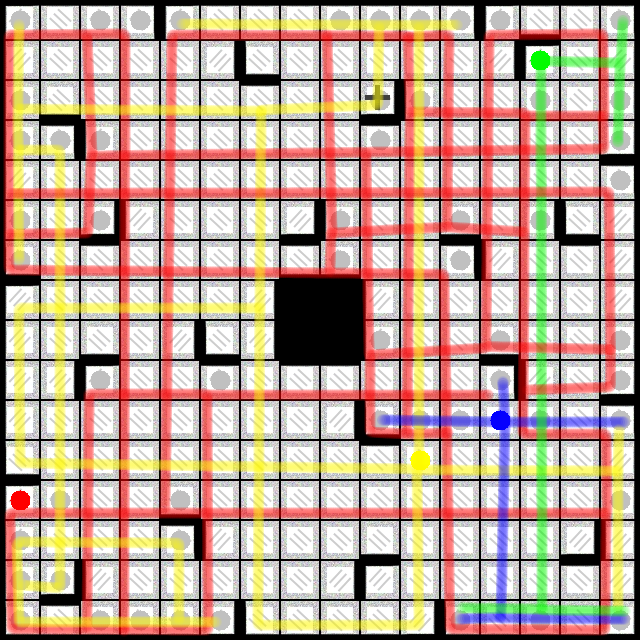
\includegraphics[width=.7\linewidth]{img/chemins_initiaux.png}
    \caption{Cartographie simplifi\'ee}
    \label{fig:itineraire}
  \end{figure}

On a le lemme suivant:\\
\begin{description}
  \item[Lemme : ] Si en construisant sa carte, un robot s'arrête sur une case atteignable \footnote{case où un robot peut s'arrêter} par un robot dont la carte est d\'ej\`a construite, alors il peut parcourir toute la carte de ce dernier.
\end{description}

\section{Recherche d'une solution}
Deux cas de figure peuvent se pr\'esenter :
\begin{itemize}
  \item[-] Soit le robot cibl\'e peut atteindre la cible; dans ce cas, il faut \'evaluer cette solution par rapport \`a un chemin utilisant d'autres robots;
  \item[-] Soit il ne l'atteint pas, auquel cas il faut obligatoirement utiliser un ou plusieurs autres robots pour trouver une solution.
\end{itemize}

Nous allons commencer par examiner la deuxi\`eme situation. Lors de la g\'en\'eration de la premi\`ere carte, le robot cibl\'e ne peut pas atteindre la cible. Il est donc n\'ecessaire de manipuler un ou plusieurs autres robots. Pour commencer, nous allons tenter de trouver une case atteignable par le robot cibl\'e et un autre robot en partant de la cible. Si de telles cases sont d\'ecouvertes, celle qui est accessible le plus rapidement sera choisie.

\subsection{Initialisation de la recherche \`a partir de la cible}
\begin{tabular}{l}
\hspace{-.1cm}g\'en\'eration $\leftarrow 0$\\
\\
\hspace{-.1cm}Pour chaque direction disponible faire\\
  \begin{tabular}{|l}
  Cr\'eer un clone\\
  Explore(clone, g\'en\'eration)\\
  \end{tabular}
  \\Masquer robot
\end{tabular}

\subsection{Exploration}
\begin{tabular*}{\textwidth}{p{.7\textwidth}}
\hspace{-.1cm}$mem$ : tableau d'entiers\\
\hspace{-.1cm}$choix \in M_{i,j} \times \mathbb{N}$\\
\hspace{-.1cm}$i = 0$\\
\\
\hspace{-.1cm}Tant que le clone n'est pas bloqu\'e faire\\
  \begin{tabular}{|l}
    Si $(M_{i,j}$ atteignable par $R_{cible})$ et $(\exists R_c | M_{i,j}$ atteignable par $R_c)$\\
    Alors $mem[i] \leftarrow (M_{i,j},d(M_{i,j},R_c))$\\
    Avancer\\
  \end{tabular}
%\\$choix \leftarrow min(mem)[0]$ \comment{r\'ecup\'eration de la case o\`u se trouve la distance minimale}
\end{tabular*}
%\comment{Ici, choix correspond \`a la case o\`u $\left(R_{c_{i,j}} | c \neq couleur(R_c)\right)$ pourra venir bloquer $R_{cible}$}
\begin{tabular*}{\textwidth}{p{.7\textwidth}}
  \\
  \hspace{-.1cm}Trier $mem$ par $d(M_{i,j},R_c)$ croissant.\\
  \hspace{-.1cm}$tmp \leftarrow M_{i,j} + max \left( d(M_{i,j},R_c) \right)$\\
  \\
  \hspace{-.1cm}Pour i de 1 \`a $|mem|$ faire\\
  \begin{tabular*}{\textwidth}{|p{.7\textwidth}}
    Si $(M_{i,j} + d(M_{i,j},R_c)) < tmp$\\
    Alors\\
    \begin{tabular*}{\textwidth}{|p{.7\textwidth}}
      $tmp \leftarrow min(tmp,M_{i,j} + d(M_{i,j},R_c)  + d(M_{i,j},C_{i,j}))$\\
    \end{tabular*}
  \end{tabular*}
\end{tabular*}
\\
\comment{algorithme incomplet, il faut encore recommencer avec de nouvelles g\'en\'erations et chercher la condition d'arr\^et notamment}

\end{document}